\chapter{Lie groups}

\begin{center}
    \vspace{-15pt}
    {\large\itshape "Groups with a notion of continuity."\par}
    \vspace{-8pt}
    {\color{gray!70}\rule{0.32\textwidth}{0.5pt}\par}
\end{center}


\ex{
    \begin{itemize}
        \item $(\mathbb{R},+)$ has a notion of closeness $\lim_{n\to\infty} a_n = b$ and a notion of continuity as we can describe paths $\gamma(-\epsilon,\epsilon)\to\mathbb{R}$
        \item $(\mathbb{R}^n,+)$, $U(N)$, $SU(N)$, $SO(N)$, $GL(N,\mathbb{R})$, $GL(N,\mathbb{C})$ are all groups with a notion of closeness and continuity
    \end{itemize}
}

Consider the 1 dimensional representations of $\mathbb{R}$, i.e. the homomorphisms 
\[\rho:(\mathbb{R},+)\to(\mathbb{C}^\times,\cdot)\]
Given $\rho(1) = c$, we can immediately conclude the following:
\begin{itemize}
    \item $\rho(n) = \rho(1+1+\cdots+1) = \rho(1)^n = c^n$
    \item $c = \rho(\frac1n \cot n) = \rho(\frac1n)^n \Rightarrow \rho(\frac1n) = c^{\frac1n}$
    \item $\rho(\frac{m}{n}) = c^{\frac{m}{n}}$
\end{itemize}

Since $\mathbb{R}$ is a vector space over $\mathbb{Q}$, it has a $\mathbb{Q}$-basis $\{1,a_i\}_{i\in I}$ with uncountable index set $I$. Then for a representation $\rho$, we have $\rho(a_i) \in \mathbb{C}^\times$ and $\rho\left(\sum_{i \in I} \lambda_i a_i\right) = \prod_{i \in I} \rho(a_i)^{\lambda_i}$ for $\lambda_i \in \mathbb{Q}$. This means that the representation is determined by the values $\{\rho(a_i)\}_{i\in I}$, which can be chosen arbitrarily. Hence, there are uncountably many 1-dimensional representations of $\mathbb{R}$. Thus representations without continuity conditions are hopeless.

\defn[matrix Lie group]{Matrix Lie groups}{
    A \textbf{matrix Lie group} is a closed subgroup of $GL(n,\mathbb{R})$. Closedness is with respect to the usual topology on $\mathbb{R}^{n^2}$.
}
\rmkb{Complex matrix groups e.g. $SU(n)$ can be viewed as a subgroup of $GL(2n,\mathbb{R})$.}

\ex{The real numbers with addition $(\mathbb{R},+)\cong \left\{\begin{pmatrix}1 & x \\ 0 & 1\end{pmatrix} : x \in \mathbb{R}\right\}$ is a matrix Lie group.}

\section{A few basics from differential geometry}

\defn[topological space]{topological space}{
    A \textbf{topological space} $X$ is characterized by a collection of subsets called the opensets,
    $\mathcal{O}(X) \subseteq \mathcal{P}(X)$ such that: 
    \begin{itemize}
        \item $\emptyset, X \in \mathcal{O}(X)$
        \item $\bigcup_{i\in I} U_i \in \mathcal{O}(X)$ for $U_i$ a family of opensets
        \item $U_1 \cap U_2 \in \mathcal{O}(X)$ for $U_1,U_2 \in \mathcal{O}(X)$
    \end{itemize}
}

\ex{
    Let $(X,d)$ be a metric space. Define $U\subseteq X$ to be open if
    \[\forall x \in U \quad \exists \, \epsilon \textgreater 0 \text{ such that } B(x,\epsilon) \coloneq \{y\in X : d(y,x) \textless \epsilon\} \subseteq U\]

}

\defn[continuous map]{continuous map}{
    A map $f:X\to Y$ between topological spaces is \textbf{continuous} if
    \[
        f^{-1}(U)\in\mathcal{O}(X) \quad \forall U\in\mathcal{O}(Y).
    \]
    If $f$ is a bijection whose inverse is also continuous, it is called a \textbf{homeomorphism}\index{homeomorphism}.
}

\defn[chart]{chart}{
    A \textbf{chart} on a topological space $X$ is a pair $(U_\alpha,\psi_\alpha)$ consisting of an open set $U_\alpha\subseteq X$ and a homeomorphism
    \[
        \psi_\alpha:U_\alpha\to V_\alpha\subseteq\mathbb{R}^n.
    \]
    For two charts $(U_\alpha,\psi_\alpha)$ and $(U_\beta,\psi_\beta)$ with $U_\alpha\cap U_\beta\neq\emptyset$, the \textbf{transition map}
    \[
        \psi_{\alpha\beta}:\tilde V_\alpha\to\tilde V_\beta
    \]
    is obtained by restricting $\psi_\alpha,\psi_\beta$ to the images $\tilde V_\alpha,\tilde V_\beta$ of the intersection $U_\alpha\cap U_\beta$. Since this is a map between subsets of $\mathbb{R}^n$, the notion of smoothness is well defined.\index{transition map}
}

\defn[atlas]{atlas}{
    An \textbf{atlas} on $X$ is a collection of charts $\{(U_i,\psi_i)\}_{i\in I}$ whose domains form an open cover of $X$:
    \[
        \bigcup_{i\in I} U_i=X.
    \]
    An atlas is \textbf{maximal}\index{atlas!maximal} if it is not contained in a larger atlas.
}

\defn[Hausdorff space]{Hausdorff space}{
    A topological space $X$ is called \textbf{Hausdorff} if
    \[
        \forall x,y\in X \text{ with } x\neq y \quad \exists\, U_x,U_y\in\mathcal{O}(X) \text{ such that } x\in U_x,\ y\in U_y,\ U_x\cap U_y=\emptyset.
    \]
}

\defn[manifold]{manifold}{
    An \textbf{$n$-dimensional (smooth) manifold} is a topological Hausdorff space equipped with a maximal atlas.
}

\rmkb{
    \textbf{Why Hausdorff?} We want unique limits. Consider
    \[
        \mathbb{R}\sqcup\mathbb{R}\,\big/\,(x_1\sim x_2 \text{ for } x_1\neq 0)
    \]
    $\rightarrow$ ``$\mathbb{R}$ with two zeros''.
    \begin{center}
    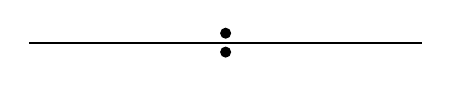
\begin{tikzpicture}[baseline]
        \draw[thick] (-2.5,0) -- (2.5,0);
        \fill (0, 0.12) circle (2pt);
        \fill (0,-0.12) circle (2pt);
    \end{tikzpicture}
    \end{center}
    This has a maximal atlas but is \emph{not} Hausdorff. Limits are not uniquely defined. Thus we require Hausdorffness to ensure that limits are well-defined.
}

\ex{
    \begin{itemize}
        \item $\mathbb{R}^n$ is a manifold; $\mathrm{id}:\mathbb{R}^n\to\mathbb{R}^n$ is an atlas. (This manifold structure is unique, except $\mathbb{R}^4$ which has $\infty$ many.)
        \item $S^1\subset\mathbb{R}^2$ defined by $x^2+y^2=1$
        is covered by the four charts

        \begin{center}
        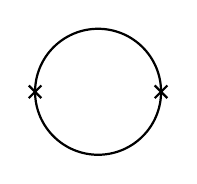
\begin{tikzpicture}
            \draw[thick] (0,0) circle (0.8);
            \draw[thick] (0.72, 0.08) -- (0.88, -0.08)  (0.72,-0.08) -- (0.88, 0.08);
            \draw[thick] (-0.72, 0.08) -- (-0.88,-0.08) (-0.72,-0.08) -- (-0.88, 0.08);
        \end{tikzpicture}
        \end{center}

        \begin{align*}
            \psi_\pm^x &: \{(x,\pm\sqrt{1-x^2})\mid x\neq\pm 1\}\longrightarrow(-1,1),\quad (x,y)\mapsto x\\
            \psi_\pm^y &: \{(\pm\sqrt{1-y^2},y)\mid y\neq\pm 1\}\longrightarrow(-1,1),\quad (x,y)\mapsto y
        \end{align*}
        $\Rightarrow$ $S^1$ is a manifold.
    \end{itemize}
}

\defn[smooth map]{smooth map}{
    Let $M,N$ be manifolds. A continuous map $f:M\to N$ is \textbf{smooth} if for all $m\in M$ there exists a chart $U_m$ containing $m$ and a chart $U_{f(m)}$ containing $f(U_m)$ such that
    \[
        \psi_{f(m)}\circ f\circ\psi_m^{-1}
    \]
    is smooth. A \textbf{diffeomorphism}\index{diffeomorphism} is a smooth map with smooth inverse.
}

\defn[derivation]{derivation}{
    For $M$ a manifold, we write $C^\infty(M)$ for the vector space of smooth functions $f:M\to\mathbb{R}$.

    For $x\in M$, a \textbf{derivation} at $x$ is a linear map
    \[
        D_x : C^\infty(M)\longrightarrow\mathbb{R}
    \]
    satisfying the Leibniz rule
    \[
        D_x(f\cdot g) = D_x(f)\cdot g(x) + f(x)\cdot D_x(g).
    \]

    Given local coordinates $(x_1,\dots,x_n)$ on a chart $U_\alpha$ containing $x$, one defines
    \[
        \frac{\partial}{\partial x_i}\bigg|_x : C^\infty(M)\longrightarrow\mathbb{R},
        \qquad
        f\longmapsto \frac{\partial}{\partial x_i}\bigg|_{\psi_\alpha(x)}\!\!(f\circ\psi_\alpha^{-1}).
    \]
    The derivations $\tfrac{\partial}{\partial x_i}\big|_x$ form a basis of the vector space of derivations at $x$.
}

\defn[tangent space]{tangent space}{
    The \textbf{tangent space} to $M$ at $x\in M$ is the vector space
    \[
        T_x M := \{\text{derivations at }x\}.
    \]
}

\ex{
    \begin{itemize}
        \item $T_x\mathbb{R}^n = \operatorname{span}\!\left\{\dfrac{\partial}{\partial x^1},\dots,\dfrac{\partial}{\partial x^n}\right\}$
        \item $T_v V = V$ for $V$ a vector space.
    \end{itemize}
}

\rmkb{
    \textbf{Tangent vectors as equivalence classes of curves.} Consider a smooth curve
    \[
        \gamma(t):(-\varepsilon,\varepsilon)\longrightarrow M, \qquad \gamma(0)=x.
    \]
    Its differential at $0$ is a linear map
    \[
        d\gamma\big|_0 : T_0(-\varepsilon,\varepsilon)\longrightarrow T_x M,
        \qquad
        \frac{\partial}{\partial t}\longmapsto d\gamma\big|_0\!\left[\frac{\partial}{\partial t}\right].
    \]
    For $F\in C^\infty(M)$ this acts as
    \[
        d\gamma\big|_0\!\left[\frac{\partial}{\partial t}\right](F)
        =
        \frac{\partial}{\partial t}\bigg|_{t=0} F(\gamma(t)).
    \]
    For $M=V$ a vector space with $T_x V = V$, writing $\gamma(t)=\gamma^1(t)x^1+\cdots+\gamma^n(t)x^n$ gives
    \[
        \frac{\partial}{\partial t}F(\gamma(t))
        =
        \frac{\partial F}{\partial x^1}\frac{\partial\gamma^1}{\partial t}+\cdots+\frac{\partial F}{\partial x^n}\frac{\partial\gamma^n}{\partial t},
    \]
    so that
    \[
        d\gamma\big|_0\!\left[\frac{\partial}{\partial t}\right] = \dot\gamma(0) \in V = T_x V.
    \]
    Hence a tangent vector at $x$ can equivalently be viewed as the velocity $\dot\gamma(0)$ of a curve through $x$.
}

\defn[differential (of a smooth map)]{differential}{
    Let $f:M\to N$ be a smooth map. It induces a linear map
    \[
        df\big|_x : T_x M \longrightarrow T_{f(x)} N,
        \qquad
        D_x \longmapsto \Bigl(h\mapsto D_x(h\circ f)\Bigr)
        \quad \forall\, h\in C^\infty(N),
    \]
    called the \textbf{differential}, or \textbf{push-forward}\index{push-forward}, of $f$. In local coordinates $x^i$ on $M$ and $y^j$ on $N$,
    \[
        \frac{\partial}{\partial x^i}\longmapsto \sum_j \frac{\partial f^j}{\partial x^i}\,\frac{\partial}{\partial y^j}.
    \]
}

\section{Lie algebras}

\defn[Lie group]{Lie group}{
    A \textbf{Lie group} is a smooth manifold $G$ equipped with a group structure such that
    \[
        \bullet : G\times G\longrightarrow G
        \qquad\text{and}\qquad
        {(\,\cdot\,)}^{-1} : G\longrightarrow G
    \]
    are smooth maps.
}

\rmkb{The Cartesian product of manifolds is (in most cases) also a manifold.}

$G$ acts on itself by conjugation
\[
    \mathrm{Ad}(g) : G\longrightarrow G, \qquad h\longmapsto ghg^{-1},
\]
which is a smooth map since Lie groups act smoothly by definition. Taking the differential at the identity gives a linear map
\[
    d\,\mathrm{Ad}(g)\big|_e : T_e G\longrightarrow T_e G,
\]
and hence a group homomorphism
\[
    \mathrm{ad} : G\longrightarrow \mathrm{Aut}(T_e G).
\]

\defn[-]{smooth representation}{
    Let $G$ be a Lie group. A \textbf{(smooth) representation}\index{representation!smooth} of $G$ is a smooth group homomorphism
    \[
        G\longrightarrow \mathrm{Aut}(V)
    \]
    for a vector space $V$.
}

\propp{
    Let $G$ be a Lie group. The map
    \[
        \mathrm{ad} : G\longrightarrow \mathrm{Aut}(T_e G),
        \qquad
        g\longmapsto d\,\mathrm{Ad}(g)\big|_e,
    \]
    is a representation of $G$, called the \textbf{adjoint action}\index{adjoint action}.
}{
    \textit{Homomorphism.} We need $\mathrm{ad}(g)\circ\mathrm{ad}(h) = \mathrm{ad}(gh)$, i.e.
    \[
        d\,\mathrm{Ad}(g)\big|_e \circ d\,\mathrm{Ad}(h)\big|_e
        =
        d\,\mathrm{Ad}(gh)\big|_e.
    \]
    This follows from $\mathrm{Ad}_g\circ\mathrm{Ad}_h = \mathrm{Ad}_{gh}$ together with the chain rule: for smooth maps $f:M\to N$ and $f':N\to O$,
    \[
        df'\big|_{f(m)}\circ df\big|_m = d(f'\circ f)\big|_m.
    \]
    Indeed, for a derivation $D_m\in T_m M$ and $h\in C^\infty(O)$,
    \begin{align*}
        \bigl(df'\big|_{f(m)}\circ df\big|_m\bigr)(D_m)[h]
        &= df'\big|_{f(m)}\bigl(D_m(h\circ f'\circ \cdot)\bigr) \\
        &= D_m(h\circ f'\circ f)
        = d(f'\circ f)\big|_m(D_m)[h].
    \end{align*}

    \textit{Identity.} $\mathrm{Ad}(e) = \mathrm{id}_G$, so $\mathrm{ad}(e) = d(\mathrm{id}_G)\big|_e = \mathrm{id}_{T_e G}$.

    \textit{Smoothness.} Follows from the smoothness of the group operations.
}

\propp{
    Let $f:G\to H$ be a Lie group homomorphism. Then $df\big|_e : T_e G\to T_e H$ satisfies
    \[
        df\big|_e \circ \mathrm{ad}_G(g) = \mathrm{ad}_H(f(g))\circ df\big|_e
        \qquad \forall\, g\in G.
    \]
}{
    We first show that $f\circ \mathrm{Ad}_G(g) = \mathrm{Ad}_H(f(g))\circ f$. For all $g,h\in G$,
    \[
        f\bigl(\mathrm{Ad}_G(g)[h]\bigr)
        = f(ghg^{-1})
        = f(g)\,f(h)\,{f(g)}^{-1}
        = \mathrm{Ad}_H(f(g))[f(h)].
    \]
    The statement then follows by differentiating both sides at the identity using $d(\,\cdot\,)\big|_e$.
}

\ex{
    Let $V$ be a finite-dimensional vector space. The group $\mathrm{Aut}(V)$ is an open subset of $\mathrm{End}(V)\cong\mathbb{R}^{2\dim V}$, so its tangent space at the identity is
    \[
        T_{\mathrm{id}}\,\mathrm{Aut}(V) \cong \mathrm{End}(V).
    \]
    The adjoint action of $\mathrm{Aut}(V)$ on $\mathrm{End}(V)$ is
    \[
        \mathrm{ad}(U) : A \longmapsto UAU^{-1}.
    \]
}

\defn[Lie bracket]{Lie bracket}{
    Let $G$ be a Lie group. The differential of $\mathrm{ad}$ at the identity gives a map
    \[
        d\,\mathrm{ad}\big|_e : T_e G \longrightarrow T_{\mathrm{id}}\,\mathrm{Aut}(T_e G) = \mathrm{End}(T_e G).
    \]
    The \textbf{Lie bracket} on $T_e G$ is defined by
    \[
        [X,Y] := d\,\mathrm{ad}\big|_e(X)[Y] \in T_e G
        \qquad \forall\, X,Y \in T_e G.
    \]
}

How do we compute $[X,Y]$?

\ex{
    Consider $G = \mathrm{Aut}(V)$, so $T_e G = \mathrm{End}(V)$. For $X\in\mathrm{End}(V)$, the curve
    \[
        \gamma_X(t) = \mathbb{1} + tX
    \]
    passes through $e$ at $t=0$ with tangent vector $X$, since $X[v] = \tfrac{\partial}{\partial t}\big|_{t=0}\gamma_X(t)[v]$.

    By definition of the Lie bracket,
    \[
        [X,Y]F
        = d\,\mathrm{ad}\big|_e(X)[Y]\,F
        = \frac{\partial}{\partial t_1}\bigg|_{t_1=0} \mathrm{ad}(\gamma_X(t_1))[Y]\,F.
    \]
    Since $\mathrm{ad}(U)$ acts by conjugation, $\mathrm{ad}(\gamma_X(t_1))[Y]\,F = Y[F({\gamma_X(t_1)}\,\cdot\,{\gamma_X(t_1)}^{-1})]$. Representing $Y$ by a curve $\gamma_Y$,
    \begin{align}
        [X,Y]F
        &= \frac{\partial}{\partial t_1}\bigg|_{t_1=0} Y\bigl[F\bigl({\gamma_X(t_1)}\,(\cdot)\,{\gamma_X(t_1)}^{-1}\bigr)\bigr] \notag\\
        &= \frac{\partial}{\partial t_1}\frac{\partial}{\partial t_2}\bigg|_{t_1=t_2=0} F\bigl({\gamma_X(t_1)}\,\gamma_Y(t_2)\,{\gamma_X(t_1)}^{-1}\bigr). \label{eq:bracket-curves}
    \end{align}
    For $G = \mathrm{GL}(n)$ with $\gamma_X(t)=\mathbb{1}+t_1 X$ and $\gamma_Y(t)=\mathbb{1}+t_2 Y$,
    \begin{align*}
        [X,Y]
        &= \frac{\partial}{\partial t_1}\frac{\partial}{\partial t_2}\bigg|_{t_1=t_2=0}
           (\mathbb{1}+t_1 X)(\mathbb{1}+t_2 Y){(\mathbb{1}+t_1 X)}^{-1}\\
        &= \frac{\partial}{\partial t_1}\frac{\partial}{\partial t_2}\bigg|_{t_1=t_2=0}
           (\mathbb{1}+t_1 X)(\mathbb{1}+t_2 Y)(\mathbb{1}-t_1 X+\mathcal{O}(t_1^2))\\
        &= XY - YX.
    \end{align*}
}

We have shown that any Lie group $G$ gives rise to a tangent space $T_e G$ equipped with a bilinear bracket
\[
    [-,-] : T_e G\otimes T_e G \longrightarrow T_e G,
\]
and that for matrix Lie groups this bracket is the commutator $[X,Y]=XY-YX$.

\propp{
    Let $f:G\to H$ be a Lie group homomorphism. Then
    \[
        {\bigl[df\big|_e X,\; df\big|_e Y\bigr]}_{T_e H}
        =
        df\big|_e\,[X,Y]_{T_e G}.
    \]
}{
    Using formula~\eqref{eq:bracket-curves},
    \begin{align*}
        {\bigl[df\big|_e X,\; df\big|_e Y\bigr]}_{T_e H} F
        &= \frac{\partial}{\partial t_1}\frac{\partial}{\partial t_2}\bigg|_{t_1=t_2=0}
           F\!\left({f(\gamma_X(t_1))}\,f(\gamma_Y(t_2))\,{f(\gamma_X(t_1))}^{-1}\right)\\
        &= \frac{\partial}{\partial t_1}\frac{\partial}{\partial t_2}\bigg|_{t_1=t_2=0}
           F\!\left(f\!\left({\gamma_X(t_1)}\,\gamma_Y(t_2)\,{\gamma_X(t_1)}^{-1}\right)\right)\\
        &= df\big|_e\,[X,Y]_{T_e G}\,F,
    \end{align*}
    where in the second step we used that $f$ is a group homomorphism, and in the third step we applied formula~\eqref{eq:bracket-curves} for~$G$.
}

\rmkb{
    For matrix Lie groups $G\leq\mathrm{GL}(n)$, the inclusion $G\hookrightarrow\mathrm{GL}(n)$ is a Lie group homomorphism, so $T_e G\subseteq\mathrm{End}(\mathbb{R}^n)$ and the bracket on $T_e G$ is the restriction of the commutator:
    \[
        {[X,Y]}_{T_e G} = XY - YX.
    \]
}

\thmp{Properties of the Lie bracket}{
    Let $G$ be a Lie group. For all $X,Y,Z\in T_e G$:
    \begin{enumerate}
        \item $[X,Y]=-[Y,X]$ \quad (antisymmetric)
        \item $[X,[Y,Z]]+[Z,[X,Y]]+[Y,[Z,X]]=0$ \quad (Jacobi identity)
    \end{enumerate}
}{
    \textbf{Antisymmetry.} We show $[X,X]=0$; antisymmetry then follows from
    \[
        0=[X+Y,X+Y]=[X,Y]+[Y,X].
    \]
    Assume $\gamma_X(t)\cdot\gamma_X(t')=\gamma_X(t+t')$ for $t,t'$ near $0$. Then in local coordinates
    \[
        \frac{\partial}{\partial t}\gamma(t)
        =\lim_{\varepsilon\to 0}\frac{\gamma(t+\varepsilon)-\gamma(t)}{\varepsilon}
        =\lim_{\varepsilon\to 0}\gamma(t)\,\frac{\gamma(\varepsilon)-\gamma(0)}{\varepsilon}
        =\gamma(t)\cdot X.
    \]
    This is a system of ODEs and hence has a unique solution near $t=0$, so $\gamma_X$ exists.
    Using the Proposition above,
    \[
        [X,X]\,F
        =\frac{\partial}{\partial t_1}\frac{\partial}{\partial t_2}\bigg|_{\substack{t_1=0\\t_2=0}}
         F\!\bigl(\gamma_X(t_1)\,\gamma_X(t_2)\,\gamma_X(-t_1)\bigr)
        =\frac{\partial}{\partial t_1}\frac{\partial}{\partial t_2}\bigg|_{\substack{t_1=0\\t_2=0}}
         F\!\bigl(\gamma_X(t_2)\bigr)
        =0,
    \]
    where we used $\gamma_X(t_1)\,\gamma_X(t_2)\,\gamma_X(-t_1)=\gamma_X(t_2)$.

    \medskip
    \textbf{Jacobi identity.} Consider
    \[
        H:T_e G\to\mathrm{End}(T_e G),\qquad X\mapsto[X,-],
    \]
    which is the differential of $G\to\mathrm{Aut}(T_e G)$. By the previous proposition,
    \[
        H([X,Y]):=[[X,Y],-]=H(X)\circ H(Y)-H(Y)\circ H(X).
    \]
    Evaluating at $Z\in T_e G$:
    \begin{align*}
        {[[X,Y],Z]}&=[X,[Y,Z]]-[Y,[X,Z]]\\
                   &=-[Z,[X,Y]]=[X,[Y,Z]]+[Y,[Z,X]],
    \end{align*}
    hence $0=[X,[Y,Z]]+[Y,[Z,X]]+[Z,[X,Y]]$.
}

\defn[Lie algebra]{Lie algebra}{\index{Jacobi identity}
    A \textbf{Lie algebra} is a vector space $\mathfrak{g}$ equipped with a linear map
    \[
        [-,-]:\mathfrak{g}\otimes\mathfrak{g}\to\mathfrak{g}
    \]
    such that for all $X,Y,Z\in\mathfrak{g}$:
    \begin{itemize}
        \item $[X,Y]=-[Y,X]$
        \item $[X,[Y,Z]]+[Z,[X,Y]]+[Y,[Z,X]]=0$ \quad (Jacobi identity)
    \end{itemize}
}

\defn[Lie algebra homomorphism]{Lie algebra homomorphism}{
    A \textbf{Lie algebra homomorphism} is a map $f:\mathfrak{g}\to\mathfrak{g}'$ such that
    \[
        f([X,Y])=[f(X),f(Y)].
    \]
}

\rmkb{
    For any Lie group, $T_e G =: \mathfrak{g}$ is a Lie algebra, and every Lie group homomorphism $G\to H$ induces a Lie algebra homomorphism $\mathfrak{g}\to\mathfrak{h}$. In particular, a representation $\rho:G\to\mathrm{Aut}(V)$ induces a Lie algebra homomorphism $\mathfrak{g}\to\mathrm{End}(V)$.
}

\defn[Lie algebra representation]{Representation of a Lie algebra}{
    Let $\mathfrak{g}$ be a Lie algebra. A \textbf{representation} of $\mathfrak{g}$ is a Lie algebra homomorphism
    \[
        \mathfrak{g}\to\mathrm{End}(V)
    \]
    for a vector space $V$.
}

\rmkb{
    Most definitions for finite groups, such as irreducible representations, carry over unchanged to Lie groups. We will not repeat them here.
}

\ex{\index{SU(2)}\index{su(2) Lie algebra@$\mathfrak{su}(2)$}
    \textbf{The Lie group $SU(2)$ and its Lie algebra $\mathfrak{su}(2)$.}
    \[
        SU(2) := \bigl\{U\in GL(2,\mathbb{C})\;\big|\; U^\dagger U=\mathbb{1},\;\det(U)=1\bigr\}
    \]
    This is not a complex Lie group (real dimension~3), even though the elements are complex.

    For $U=\begin{pmatrix}a&b\\c&d\end{pmatrix}$ and $U^\dagger=\begin{pmatrix}\bar{a}&\bar{c}\\\bar{b}&\bar{d}\end{pmatrix}$,
    \[
        U^\dagger U =
        \begin{pmatrix}
            \bar{a}a+\bar{c}c & \bar{a}b+\bar{c}d \\
            \bar{b}a+\bar{d}c & \bar{b}b+\bar{d}d
        \end{pmatrix}
        = \begin{pmatrix}1&0\\0&1\end{pmatrix},\qquad ad-bc=1.
    \]
    All solutions are of the form
    \[
        \begin{pmatrix}\alpha&-\bar{\beta}\\\beta&\bar{\alpha}\end{pmatrix},
        \qquad |\alpha|^2+|\beta|^2=1,\tag{$**$}
    \]
    hence $\dim SU(2)=3$.

    For every $U\in SU(2)$, there exists $V\in U(2)$ such that
    \[
        VUV^{-1}=\begin{pmatrix}\alpha&0\\0&\bar\alpha\end{pmatrix}.
    \]
    Setting $V'={(\det V)}^{-1/2}V$ gives $V'\in SU(2)$, so the conjugacy classes are labelled by
    $\alpha\in U(1)/\mathbb{Z}_2\cong\mathbb{R}/\pi\mathbb{R}$.

    Writing $\alpha=a+ib$ and $\beta=c+id$ with $a,b,c,d\in\mathbb{R}$, condition~($**$) gives
    \[
        a^2+b^2+c^2+d^2=1,
    \]
    so $SU(2)\cong S^3$ as a manifold.
    With this parameterisation,
    \[
        U = \begin{pmatrix}a+ib&c+id\\c-id&a-ib\end{pmatrix}
        = a\underbrace{\begin{pmatrix}1&0\\0&1\end{pmatrix}}_{\mathbf{1}}
        + b\underbrace{\begin{pmatrix}i&0\\0&-i\end{pmatrix}}_{\mathbf{i}}
        + c\underbrace{\begin{pmatrix}0&1\\1&0\end{pmatrix}}_{\mathbf{j}}
        + d\underbrace{\begin{pmatrix}0&i\\-i&0\end{pmatrix}}_{\mathbf{k}},
    \]
    so $SU(2)$ is also the group of unit quaternions.\index{quaternion!unit}

    \medskip\noindent\textbf{Connection to $SO(3)$.}\quad\index{double cover}\index{Spin(3)@$\mathrm{Spin}(3)$}
    The submanifold $a=0$ is diffeomorphic to $S^2$ and preserved under conjugation, giving a map
    \[
        SU(2)=\mathrm{Spin}(3)\longrightarrow SO(3)\qquad\text{(not a bijection),}
    \]
    with kernel $\{1,-1\}$, and $SO(3)=SU(2)/\mathbb{Z}_2$ is a double cover.
    Since $SU(2)$ and $SO(3)$ differ only by $-1$, which is not near the identity, the Lie algebras $\mathfrak{su}(2)$ and $\mathfrak{so}(3)$ are the same.

    \medskip\noindent\textbf{The Lie algebra $\mathfrak{su}(2)$.}\quad\index{skew-Hermitian matrix}
    $\mathfrak{su}(2)$ consists of traceless skew-Hermitian matrices ($A=-A^\dagger$), with basis
    \[
        X=\begin{pmatrix}0&i\\i&0\end{pmatrix},\qquad
        Y=\begin{pmatrix}0&1\\-1&0\end{pmatrix},\qquad
        Z=\begin{pmatrix}i&0\\0&-i\end{pmatrix}.
    \]
    The bracket satisfies $[X,Y]=2Z$ and cyclic permutations.

    \medskip\noindent\textbf{Exponential map.}\quad\index{exponential map}
    For $A\in\mathrm{Mat}(2,\mathbb{C})$, the matrix exponential is $\exp(A)=\sum_{n=0}^\infty\frac{1}{n!}A^n$.
    For $A\in\mathfrak{su}(2)$ (so $A^\dagger=-A$ and $\mathrm{tr}(A)=0$):
    \begin{itemize}
        \item ${\exp(A)}^\dagger\exp(A)=\exp(A^\dagger)\exp(A)=\exp(\underbrace{A^\dagger+A}_{=\,0})=\mathbb{1}$,
        \item $\det(\exp(A))=\exp(\mathrm{tr}(A))=1$,
    \end{itemize}
    so $\exp\colon\mathfrak{su}(2)\to SU(2)$ is a smooth map. Setting $\gamma_A(t):=\exp(tA)$ satisfies
    $\gamma_A(t+t')=\gamma_A(t)\gamma_A(t')$.
    Since ${(U^\dagger AU)}^n=U^\dagger A^n U$, we have $U^\dagger\exp(A)U=\exp(U^\dagger AU)$,
    so every conjugacy-class representative
    \[
        \begin{pmatrix}\alpha&0\\0&\bar\alpha\end{pmatrix}
        =\exp\!\begin{pmatrix}ix&0\\0&-ix\end{pmatrix},
        \qquad\alpha=e^{ix},
    \]
    is in the image, hence $\exp\colon\mathfrak{su}(2)\to SU(2)$ is surjective.

    For a representation $\rho\colon\mathfrak{su}(2)\to\mathrm{End}(V)$, one can try to define
    $\rho(\exp(A)):=\exp(\rho(A))$ for $g=\exp(A)$, but this is not well defined in general.
}

\rmkb{
    The local solution $\gamma_X$ extends to all of $\mathbb{R}$ via
    \[
        \hat{\gamma}_X:\mathbb{R}\to G,\qquad \hat{\gamma}_X(t):={\gamma_X\!\left(\tfrac{t}{n}\right)}^{\!n},
    \]
    which is a Lie group homomorphism.
}

\defn[one-parameter subgroup]{1-parameter subgroup}{
    A \textbf{1-parameter subgroup} of $G$ is a Lie group homomorphism $\mathbb{R}\to G$. These are in bijection with $\mathfrak{g}$.
}

\defn[exponential map]{Exponential map}{
    Let $G$ be a Lie group with Lie algebra $\mathfrak{g}$. The \textbf{exponential map} is
    \[
        \exp:\mathfrak{g}\to G,\qquad X\mapsto\gamma_X(1)\in G.
    \]
    For matrix Lie groups this coincides with the matrix exponential $\exp(A)=\sum_{i=0}^\infty\frac{A^i}{i!}$.
}

\rmkb{
    The differential $d\exp\big|_0:\mathfrak{g}\to\mathfrak{g}$ is the identity. This implies that $\exp$ is a diffeomorphism when restricted to small neighbourhoods of $0\in\mathfrak{g}$ and $e\in G$.
}

\rmkb{
    There is a formula for products in $G$ near $e$ in terms of the Lie bracket: the Baker-Campbell-Hausdorff formula.\index{Baker-Campbell-Hausdorff formula}
}

\propp{
    Let $\psi:G\to H$ be a Lie group homomorphism. Then $\psi\circ\exp_G=\exp_H\circ\,d\psi\big|_e$, i.e., the following diagram commutes:
    \[
    \begin{tikzpicture}[baseline=(current bounding box.center), >=Stealth]
        \node (g) at (0,1.5) {$\mathfrak{g}$};
        \node (h) at (3,1.5) {$\mathfrak{h}$};
        \node (G) at (0,0) {$G$};
        \node (H) at (3,0) {$H$};
        \draw[->] (g) -- node[above] {\small$d\psi\big|_e$} (h);
        \draw[->] (g) -- node[left]  {\small$\exp_G$} (G);
        \draw[->] (h) -- node[right] {\small$\exp_H$} (H);
        \draw[->] (G) -- node[below] {\small$\psi$} (H);
    \end{tikzpicture}
    \]
}{
    Consider $\gamma_X:\mathbb{R}\to G$. Then $\psi\circ\gamma_X$ is a group homomorphism $\mathbb{R}\to H$ (as a composition of group homomorphisms) with tangent vector $d\psi\big|_e[X]$ at $t=0$. By the bijection between 1-parameter subgroups and $\mathfrak{h}$, it follows that $\psi\circ\gamma_X=\gamma_{d\psi|_e[X]}$, and
    \[
        \psi(\exp(X))=\psi(\gamma_X(1))=\gamma_{d\psi|_e[X]}(1)=\exp\!\bigl(d\psi\big|_e[X]\bigr).
    \]
}

\defn[path-connected manifold]{Path-connected and simply connected manifolds}{\index{simply connected manifold}
    A manifold $M$ is \textbf{(path-) connected} if for each pair of points $m,n\in M$ there exists a continuous map $\gamma:[0,1]\to M$ with $\gamma(0)=m$ and $\gamma(1)=n$.

    $M$ is called \textbf{simply connected} if for each pair of paths $\gamma,\gamma'$ with $\gamma(0)=\gamma'(0)=m$ and $\gamma(1)=\gamma'(1)=n$, there exists a continuous map $H:[0,1]\times[0,1]\to M$ such that
    \begin{itemize}
        \item $H(0,t)=\gamma(t)$
        \item $H(1,t)=\gamma'(t)$
        \item $H(x,0)=m$
        \item $H(x,1)=n$
    \end{itemize}

    \begin{center}
    \begin{tikzpicture}[>=Stealth]
        \draw[rounded corners=35pt] (7,-1)--(4.2,-1)--(2,-2)--(0,0)--(2,2)--(4.2,1)--(7,1);
        \draw (1.5,0.2) arc (175:315:1cm and 0.5cm);
        \draw (3,-0.28) arc (-30:180:0.7cm and 0.3cm);
        \draw (7.5,0) arc (0:360:0.5cm and 1cm);
        \node at (20:5) {$M$};
        \filldraw (0.8, 0.4) circle (2pt) node[above left=1pt] {$m$};
        \filldraw (4.0, 0.3) circle (2pt) node[above right=1pt] {$n$};
        \draw[->,thick] (0.8,0.4) to[out=55,in=175] (2.4,1.05) to[out=-5,in=115] (4.0,0.3);
        \node at (2.3,1.3) {$\gamma$};
        \draw[->,thick] (0.8,0.4) to[out=-45,in=195] (2.4,-0.65) to[out=15,in=230] (4.0,0.3);
        \node at (2.3,-0.88) {$\gamma'$};
    \end{tikzpicture}
    \end{center}
}

\ex{
    \begin{itemize}
        \item $\mathbb{R}^n$ is simply connected.
        \item $S^1$ is connected but not simply connected.
        \item $SU(n)$ for $n\geq 2$ is simply connected.
    \end{itemize}
}

\thmp{Lie's 1st Theorem}{\index{Lie's theorems!first}
    Let $G$ be a connected Lie group. Two Lie group homomorphisms $\psi,\psi':G\to H$ are equal if $d\psi\big|_e = d\psi'\big|_e$.
}{
    By the local diffeomorphism property of $\exp$ and the identity $\psi\circ\exp_G=\exp_H\circ d\psi|_e$, the condition $d\psi\big|_e=d\psi'\big|_e$ implies $\psi=\psi'$ on a neighbourhood of $e$. It therefore suffices to show that every $g\in G$ is a product of elements from any neighbourhood $U$ of $e$.

    Let $\Gamma\subseteq G$ be the subgroup generated by $U$. Since $\Gamma=\bigcup_{h\in\Gamma}U\cdot h$, $\Gamma$ is a union of open sets and hence open. Letting $\Gamma'=G\setminus\Gamma$, for any $h'\in\Gamma'$ the coset $U\cdot h'\subseteq\Gamma'$ (otherwise $u\cdot h'\in\Gamma$ would imply $h'=u^{-1}(u\cdot h')\in\Gamma$, a contradiction), so
    \[
        \Gamma' = \bigcup_{h'\in\Gamma'} U\cdot h'
    \]
    is likewise open. Thus $G=\Gamma\sqcup\Gamma'$ is a partition into two disjoint open sets.

    If $\Gamma'\neq\emptyset$, pick $h\in\Gamma$ and $h'\in\Gamma'$. Since $G$ is path-connected, there exists $\gamma:[0,1]\to G$ with $\gamma(0)=h$ and $\gamma(1)=h'$. Then
    \[
        [0,1]=\gamma^{-1}(\Gamma)\cup\gamma^{-1}(\Gamma')
    \]
    is a partition of $[0,1]$ into two disjoint open non-empty sets, contradicting the connectedness of $[0,1]$. Hence $\Gamma'=\emptyset$, i.e.\ $\Gamma=G$.
}

\thm{Lie's 2nd Theorem}{\index{Lie's theorems!second}
    Let $G$ be a simply connected Lie group. Then there is a one-to-one correspondence between Lie group homomorphisms $\psi:G\to H$ and Lie algebra homomorphisms $\Psi:\mathfrak{g}\to\mathfrak{h}$.
}

\thm{Lie's 3rd Theorem}{\index{Lie's theorems!third}
    For each finite-dimensional real Lie algebra $\mathfrak{g}$ there exists a simply connected Lie group $G$ with Lie algebra $\mathfrak{g}$.
}

\rmkb{
    $G$ in the above is unique: if $G'$ is another simply connected Lie group with Lie algebra $\mathfrak{g}$, then $\mathrm{id}:\mathfrak{g}\to\mathfrak{g}$ lifts to a diffeomorphism $G\xrightarrow{\sim}G'$.

    \medskip\noindent\textbf{Example.} $(\mathbb{R},+)\xrightarrow{\,\exp\,}U(1)$ is a Lie algebra isomorphism (both have Lie algebra $\mathbb{R}$), but the only Lie group homomorphism $U(1)\to\mathbb{R}$ is the constant map at $0$, since $U(1)\cong S^1$ is not simply connected.
}

\corp{
    For a simply connected Lie group $G$ there is a bijection between representations of $G$ and representations of $\mathfrak{g}$.
}{
    A representation $\rho:G\to\mathrm{Aut}(V)$ is a Lie group homomorphism, which by Lie's 2nd Theorem corresponds bijectively to a Lie algebra homomorphism $\mathfrak{g}\to\mathrm{End}(V)$, i.e.\ a representation of $\mathfrak{g}$.
}{}

